\chapter{Environment}\label{chap:context}

\begin{sectionIntro}
    This chapter will describe essential facts about my internship, such as
    which company I did my internship in and on what did I worked.
\end{sectionIntro}

\section{Company}

\subsection{Celad}
Celad is an IT consulting company with about 800 employees. It was created in Toulouse
and it's headquarters are still in Toulouse.
The major activities of Celad cover:
\begin{description}
    \item [Information systems] such as solutions for E-banking, E-business, mobile applications.
    \item [Embedded sector] such as real-time, electronics, and aerospace.
\end{description}
One of its biggest clients in the embedded sector in Toulouse is Intel.
I did my internship as a contractor for Intel via Celad.

\subsection{Intel}
Intel Corporation is the world’s largest semiconductor chip maker. They
introduced the first microprocessor in 1971 and have been the world leader in
silicon innovation since.
Following a strategy to extend the Intel Architecture to new market segments,
they are delivering smartphones and tablets powered by Intel chipsets.

Some key figures of Intel:
\begin{itemize}
\item Leading manufacturer of computer, networking and communications
  products,
  \item 300 Facilities in 50 countries,
  \item Over \$35B in Annual Revenues from customers in over 120
    countries,
\item 23 Consecutive years of positive net income,
\item Approximately 80,000 employees,
\item 43,000 technical degrees, 12,000 Masters in Science, 4,000
  PhD’s, 4,000 MBA’s,
  \item One of the top ten most valuable brands in the world for 10
    consecutive years,
\item Invests \$100 Million each year in education across more than 50
  countries,
\item One of the top ten Linux \gls{kernel} contributors.
\end{itemize}


\subsection{Intel Audio feature team in Toulouse}
The team I worked with is the Audio feature team, in Toulouse.
They are responsible for the Audio \gls{hal} and the interface between the
librairies and the \gls{android} \gls{kernel}.


\section{Android}
During my internship, I worked on the \gls{android} platform.
Let's have an overview of the \gls{android} architecture to understand where
the Audio \gls{hal} is placed within this platform.

\subsection{Global Android architecture}

On the figure \ref{fig:archi}, we can see the Audio \gls{hal} between the
Linux \gls{kernel} and the libraries layers.
\begin{figureGraphics}{Global Android architecture}{fig:archi}
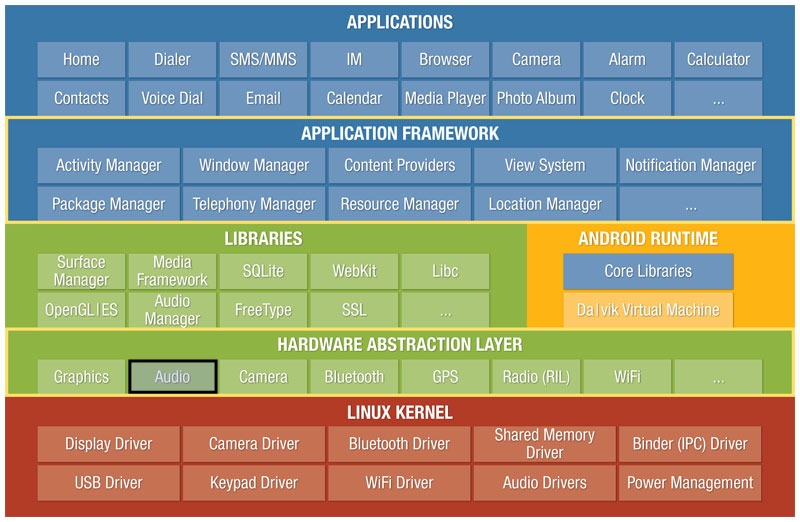
\includegraphics[width=\textwidth]{./src/img/android-archi-audio-hal.jpeg}
\end{figureGraphics}

Within the Audio feature team in Toulouse, we are mainly focused around the Audio \gls{hal}.

\subsection{Intel Audio HAL}
Intel's Audio \gls{hal} for Android platforms is based around a generic, plugin-based solution: the \gls{pfw}.
It runs in the \emph{userland}, which is easier to maintain than kernel-space code.
Since this solution is plugin-based, it is easy to extend to add more subsystems if needed.

There is an overview of the Intel Audio \gls{hal} on figure \ref{fig:hal} below.
\begin{figureGraphics}{Simplified view of Intel Audio HAL}{fig:hal}
\includegraphics[height=0.5\textheight]{./src/img/hal-architecture.pdf}
\end{figureGraphics}
Two different instances of \gls{pfw} are used to communicate between the
different managers used in the \gls{hal}.

Some requirements of the Intel Audio \gls{hal}:
\begin{itemize}
    \item Since the audio system needs to be tuned by the tuning engineers, the \gls{hal} should be configurable.
        It would have been very painful to recompile the code at each time it is needed to adapt the value of a mixer!
    \item Since the \gls{hal} needs to \emph{abstract} the hardware variations, it should also be scalable. It should be
        easy to support new hardware.
\end{itemize}

The \gls{pfw} is a way to fulfill those requirements.

\section{Parameter-framework}
\label{sec:parameter-framework}
During a phone call, the smartphone isn't just transmitting the sound received from the microphone. Various algorithms are
enabled on the audio signal which is transmitted and received.
Those algorithms have a lot of parameters, which can change depending on the use case: whether we are in a phone call,
or listing to some music. Furthermore, those parameters are \emph{often hardware dependent}.

The \gls{pfw} was born to manage easily those multiple parameters in a scalable way.

\subsection{Some concepts}
In this section we are going to discover the concepts which make the
\gls{pfw} such a powerful tool.

\subsubsection{Structure}
The \gls{pfw} is first of all a hierarchical tree of parameters.
On figure \ref{fig:pfwtree} we can see an example of audio tree.

\begin{figureGraphics}{Parameter framework tree example}{fig:pfwtree}
    \fbox{\begin{minipage}{6cm}
            \dirtree{%
                .1 audio.
                    .2 microphone.
                        .3 echo\_cancellation.
                            .4 enable.
                            .4 configuration.
                                .5 gain.
                                .5 coefficient.
                    .2 speaker.
                        .3 equalizer.
                            .4 enable.
                            .4 configuration.
                                .5 filter.
                                .5 coefficient.
            }
    \end{minipage}}
\end{figureGraphics}

These structures are stored in \gls{xml} files. This is great because it implies that we don't need
to recompile the \gls{pfw} when changing the structure we are describing.

In listing \ref{lst:pfwstructure}, when can see the \gls{xml} structure file
describing the tree from figure \ref{fig:pfwtree}.

\begin{code}[language=pfwXml, caption=Structure file example snippet, label=lst:pfwstructure]
<!--snippet-->
<ComponentType Name="echo_cancellation">
    <BooleanParameter Name="enable"/>
    <ParameterBlock Name="configuration">
        <IntegerParameter Name="gain" Size="8"/>
        <IntegerParameter Name="coefficient" Size="8"/>
    </ParameterBlock>
</ComponentType>
<!--snippet-->
\end{code}

\subsubsection{Settings}
The \gls{pfw} is also able to change multiple parameters without any manual action, depending on the context.
The context is defined using a set of criteria. Those criteria are variables which can take a set of defined values.
For example, a criteria called \emph{Output Device} can take several values such as \emph{Speaker} or \emph{Headset}.

Depending on the value of those criteria, the \gls{pfw} can automatically apply a set of values towards
multiple parameters.
On listing \ref{lst:pfwsettings} we can see an example of setting file.

\begin{code}[language=pfwLang, caption=Settings file example, label=lst:pfwsettings]
Domain:
    Conf: SpeakerWithEchoCancel
        OutputDevice Is Speaker
        Component: audio/speaker/
            echo_cancellation/enable = true
            configuration/gain = 2
            configuration/coefficient = 3
        # -- snippet --
    Conf: HeadsetWithEchoCancel
        OutputDevice Is Headset
        Component: audio/headset/
            echo_cancellation/enable = true
            configuration/gain = 3
            configuration/coefficient = 4 # arbitrary values
        # -- snippet --
\end{code}

\subsubsection{Extensibility}
Since the \gls{pfw} is \emph{plugin-based}, it is easy to extend it's functionality to other usages than Audio, such
as Camera, or Bluetooth.


\subsection{Topic of my internship}
I worked within the Intel Audio development team, as an \emph{agile
software developer}. The team is customers oriented, using \gls{scrum}
methodology (see chapter \ref{chap:organisation}). My tasks
within the team were focused around enhancing and open-sourcing the \gls{pfw} on
\gls{GitHub}\footnote{\url{www.github.com/01org/parameter-framework}} to give the team some
visibility and advertise its work.

\section{Workflow and environment}
In this section, we will cover my daily workflow. This helps
to understand how I proceeded during my whole internship.

\begin{figureGraphics}{Developer workflow}{fig:workflow}
    \includegraphics[height=0.6\textheight]{./src/img/workflow.pdf}
\end{figureGraphics}

This workflow is the same for every developer of the team. It is
detailed in the sub sections below.

\subsection{Development}
Since compiling the Android source tree requires a lot of computing power,
most of developers of our team are working remotely, via ssh.
The server we are connecting to is far more powerful than the desktops we use.
With it 32 cores and it's 2 TeraBytes of SSD, compilation time was far less time-consuming
than compiling locally!
This server also helps to have the same developer environment to avoid
time-consuming installations on local machines.

Working remotely on that server constraints developers to use command line programs only.
During my internship, I sharpened my skills in \gls{vim} and discovered \gls{tmux}.
On the figure \ref{fig:setup} below, there is a screenshot of my development setup at Intel.

\begin{figureGraphics}{Development setup with vim and tmux}{fig:setup}
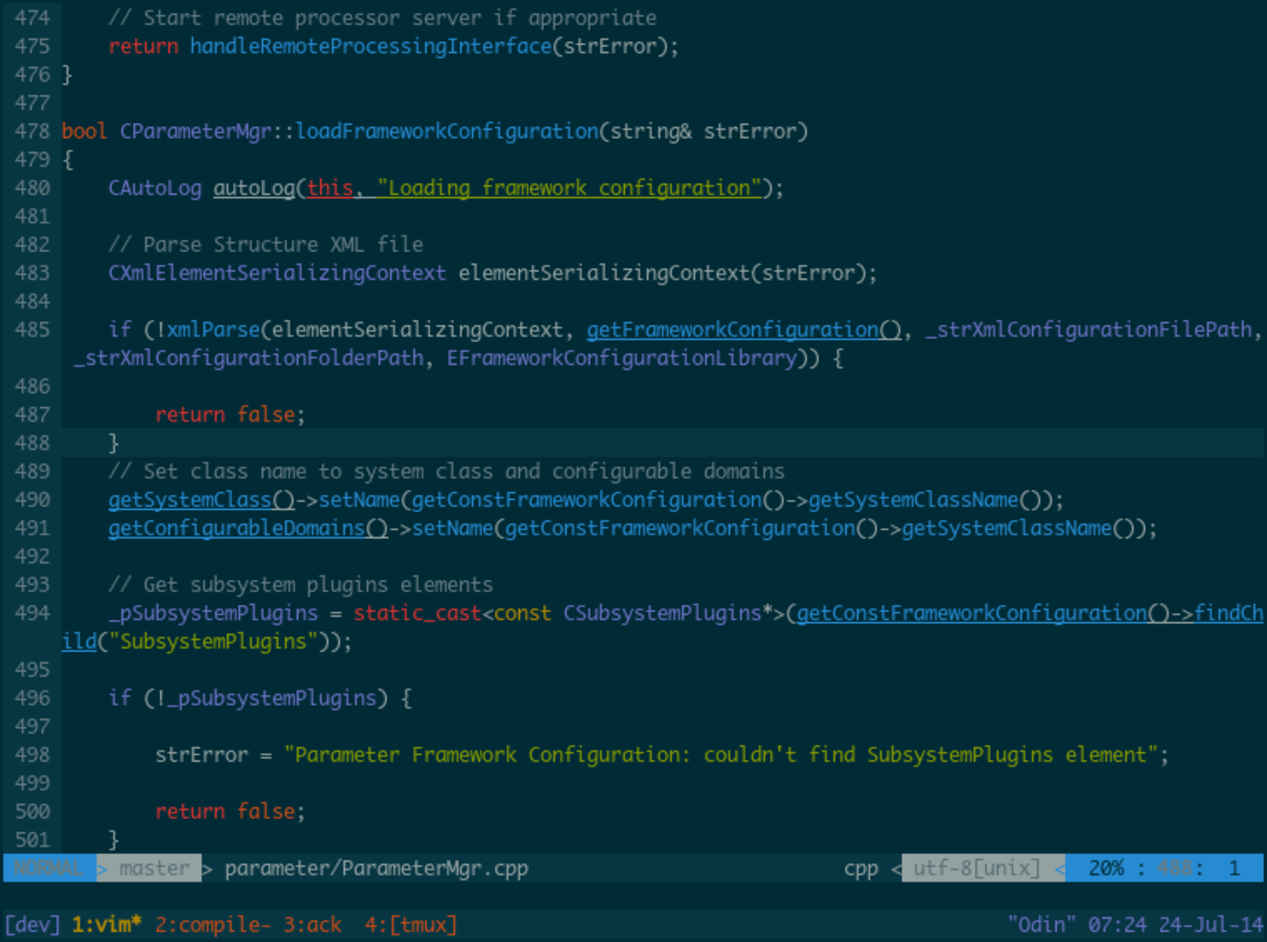
\includegraphics[width=\textwidth]{./src/img/setup.pdf}
\end{figureGraphics}

When the code is ready, I pushed it via \gls{git} on \gls{gerrit} to be reviewed.

\subsection{Git}
\gls{git} is a distributed revision control system initially designed for kernel
development. Given that fact, it can be used in environment which have large
code bases, such as \gls{android}. We use \gls{git} on daily basis at Intel for the
code delivered to customers and for the internal tools.

\subsection{Code quality}
Code quality matters. Clean code eases maintenance and is less error-prone.
Those facts are driving the team that I worked with at Intel. Naturally, all the
patches I have delivered during my internship have been reviewed and meet the
expected quality. Those reviews are done with the official \gls{android} review tool which is \gls{gerrit}.

I have done some code review myself during this internship. It helps a lot to
understand how other people work. Viewing other peoples code also makes me come
up with new ideas to improve my own work.

\subsection{Submission to gatekeeping team}
After the code is ready and validated by the development team, it is submitted towards the gatekeeping team.
They are responsible for testing complicated uses cases and they ensure there is no regression nor sound side effects
due to the modifications the development team made.

